\documentclass[xcolor=pdftex,svgnames,table]{beamer}
\usepackage{latexsym,amssymb,amsmath,stmaryrd}
\usepackage[utf8]{inputenc}
\usepackage[T1]{fontenc}
\usepackage[francais]{babel}
\usepackage{pgf}
\usepackage{tikz}
\usetikzlibrary{arrows,patterns,plotmarks,shapes,snakes,er,3d,automata,%
backgrounds,topaths,trees,petri,mindmap}
\usepackage{pgfbaseimage}
\usepackage{ifpdf}
\ifpdf
\usepackage{graphicx}
\else
%\usepackage[dvips]{graphicx}
\usepackage{pstricks,pst-tree,pst-node}
\newpsobject{showgrid}{psgrid}{subgriddiv=1,griddots=10,gridlabels=6pt}
\fi
\usepackage{moreverb}
\usepackage[normalem]{ulem}
\usepackage{version}
\usepackage{url}
\usepackage{multicol}
\usepackage{listings}
\lstset{
  language=[ANSI]C, 
%  gobble=2, 
%  escapeinside="", 
  basicstyle=\ttfamily, 
%  directivestyle=\color{Fuchsia},
  identifierstyle = \color{DarkOrange},
  keywordstyle=\color{DarkGreen}, 
  commentstyle=\color{red}, 
%  numbers=left, 
%  numbersep=5pt, 
%  numberstyle=\scriptsize, 
%  moredelim=[is][\color{gray}\itshape]{/*}{*/}, 
%  moredelim=[is][\alert]{/+}{+/}, 
%  morecomment=[is]{/=}{=/}, 
%  morecomment=[in]{comment=}{,} 
%  fancyvrb=true 
} 

\newcommand{\binaire}[1]{\ensuremath{\underline{#1}}}
\newcommand{\C}[1]{\texttt{#1}}
\newcommand{\bbbn}{\ensuremath{\mathbb{N}}}
%%%%%%%%%%%%%%%%%%%%%%%%%%%%%%%%%%%%%%%%%%%%%%%%%%%%%%%%%%%%%%%%
%% ccBeamer 0.1, 2007-07-02                                   %%
%% Written by Sebastian Pipping <webmaster@hartwork.org>      %%
%% ---------------------------------------------------------- %%
%% Licensed under Creative Commons Attribution-ShareAlike 3.0 %%
%% http://creativecommons.org/licenses/by-sa/3.0/             %%
%%%%%%%%%%%%%%%%%%%%%%%%%%%%%%%%%%%%%%%%%%%%%%%%%%%%%%%%%%%%%%%%


%% Images
\newcommand{\CcImageBy}[1]{%
	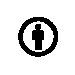
\includegraphics[scale=#1]{creative_commons/cc_by_30}%
}
\newcommand{\CcImageCc}[1]{%
	
\includegraphics[scale=#1]{creative_commons/cc_cc_30}%
}
\newcommand{\CcImageDevNations}[1]{%
	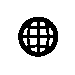
\includegraphics[scale=#1]{creative_commons/cc_dev_nations_30}%
}
\newcommand{\CcImageNc}[1]{%
	
\includegraphics[scale=#1]{creative_commons/cc_nc_30}%
}
\newcommand{\CcImageNd}[1]{%
	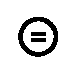
\includegraphics[scale=#1]{creative_commons/cc_nd_30}%
}
\newcommand{\CcImagePd}[1]{%
	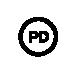
\includegraphics[scale=#1]{creative_commons/cc_pd_30}%
}
\newcommand{\CcImageSa}[1]{%
	
\includegraphics[scale=#1]{creative_commons/cc_sa_30}%
}
\newcommand{\CcImageSampling}[1]{%
	
\includegraphics[scale=#1]{creative_commons/cc_sampling_30}%
}
\newcommand{\CcImageSamplingPlus}[1]{%
	
\includegraphics[scale=#1]{creative_commons/cc_sampling_plus_30}%
}


%% Groups
\newcommand{\CcGroupBy}[1]{% zoom
	\CcImageBy{#1}%
}
\newcommand{\CcGroupByNc}[2]{% zoom, gap
	\CcImageBy{#1}\hspace*{#2}\CcImageNc{#1}%
}
\newcommand{\CcGroupByNcNd}[2]{% zoom, gap
	\CcImageBy{#1}\hspace*{#2}\CcImageNc{#1}\hspace*{#2}\CcImageNd{#1}%
}
\newcommand{\CcGroupByNcSa}[2]{% zoom, gap
	\CcImageBy{#1}\hspace*{#2}\CcImageNc{#1}\hspace*{#2}\CcImageSa{#1}%
}
\newcommand{\CcGroupByNd}[2]{% zoom, gap
	\CcImageBy{#1}\hspace*{#2}\CcImageNd{#1}%
}
\newcommand{\CcGroupBySa}[2]{% zoom, gap
	\CcImageBy{#1}\hspace*{#2}\CcImageSa{#1}%
}
\newcommand{\CcGroupDevNations}[1]{% zoom
	\CcImageDevNations{#1}%
}
\newcommand{\CcGroupNcSampling}[2]{% zoom, gap
	\CcImageNc{#1}\hspace*{#2}\CcImageSampling{#1}%
}
\newcommand{\CcGroupPd}[1]{% zoom
	\CcImagePd{#1}%
}
\newcommand{\CcGroupSampling}[1]{% zoom
	\CcImageSampling{#1}%
}
\newcommand{\CcGroupSamplingPlus}[1]{% zoom
	\CcImageSamplingPlus{#1}%
}


%% Text
\newcommand{\CcLongnameBy}{Attribution}
\newcommand{\CcLongnameByNc}{Attribution-NonCommercial}
\newcommand{\CcLongnameByNcNd}{Attribution-NoDerivs}
\newcommand{\CcLongnameByNcSa}{Attribution-NonCommercial-ShareAlike}
\newcommand{\CcLongnameByNd}{Attribution-NoDerivs}
\newcommand{\CcLongnameBySa}{Attribution-ShareAlike}

\newcommand{\CcNote}[1]{% longname
	This work is licensed under the \textit{Creative Commons #1 3.0 License}.%
}

\usetheme{classic}
\newcommand{\nowrite}{\put(10,-4){\includegraphics[scale=.05]{creative_commons/nopencil}}}
\newcommand{\youwrite}{\put(10,-4){
\includegraphics[scale=.05]{creative_commons/pencil}}}
\newcommand{\writethat}{
\includegraphics[scale=.05]{creative_commons/pencil}}
\newcommand{\aemporter}{\put(10,-6){
\includegraphics[scale=.05]{creative_commons/szymonraj_Shopping_bag}}}


%%% Titre -- cours 5
\title{Bases de programmation. -- Cours 5.\\ Structurer les données}
\author{Pierre Boudes}
\date{\today}

%\includeonlyframes{current}

\begin{document}

%% Page de titre et licence CC.
\begin{frame}
        \titlepage
        \vfill
        \begin{center}
                \CcGroupByNcSa{0.83}{0.95ex}\\[2.5ex]
                {\tiny\CcNote{\CcLongnameByNcSa}}
                \vspace*{-2.5ex}
        \end{center}
\end{frame}


%%%%%%%%%%%%%%%%%%%%
\section[Plan]{}
\frame[label=plan]{\tableofcontents}
\section[Types char et double]{Types char et double}
\subsection{Représentation des réels en virgule flottante}
\begin{frame}
    \frametitle{Représentation des réels en virgule flottante}
    \begin{itemize}
    \item La représentation informatique usuelle des réels s'inspire de la
      notation scientifique :
      \begin{align*}
        \pi &= 3,141592653589793\tag{pi}\\
        -700 \text{ milliards} &= -7 \times 10^{11}\tag{Paulson}\\
        h &= 6,626068 \times 10^{-34} \tag{Planck}\\
        \text{Univers} &= 1 \times 10^{80}  \tag{Atomes}
      \end{align*}\pause
\vspace{-.8cm}
\item Les bits sont séparés en :
  \begin{itemize}
  \item bit de signe\hfill (1 bit)
  \item mantisse \hfill (53 bits)
  \item exposant \hfill (11 bits)
  \end{itemize}\pause
\item En \textbf{double} précision (64 bits) :
  \begin{itemize}
\item exposant : entre $10^{-308}$ et $10^{308}$ (environ).
\item mantisse : 16 chiffres décimaux (environ).
  \end{itemize}\pause
\item Infini positif, infini négatif.
\item NaN : not a number.
    \end{itemize}
\end{frame}


\subsection[Types char, double et E/S]{Types et entrées sorties}
\begin{frame}
  \frametitle{Type double en C et entrées/sorties associées}

  \begin{itemize}
  \item Type des entiers relatifs  \alert{\C{int}}  (rappel) :
    \begin{itemize}
    \item Déclaration et initialisation : \C{int n = -23;}.
    \item Représentation en complément à deux.
    \item E/S : \alert{\C{\%d}}.
    \end{itemize}
  \item Les booléens \alert{\C{bool}}, sont en réalité des \C{int}
\item Type des réels \alert{\C{double}} :
  \begin{itemize}
    \item Déclaration et initialisation : \C{double x = 3.14e-3;}.
    \item Représentation en virgule flottante sur 64 bits.
    \item E/S : \alert{\C{\%lg}} (mais plutôt \C{\%g} avec \C{printf}).
    \item \alert{Attention :} toujours mettre le point (équivalent
      anglais de la virgule) pour les constantes réelles (\C{1.0}).
    \end{itemize}
  \end{itemize}
\end{frame}

\begin{frame}
  \begin{block}{Entiers}
\C{int n;\\
...\\
printf("Entrer un nombre entier$\backslash$n");\\
scanf("\%d", \alert{\&}n);}
  \end{block}\pause

\begin{block}{Réels}
\C{double x;\\
...\\
printf("Entrer un nombre reel$\backslash$n");\\
scanf("\%lg", \alert{\&}x);\\ \pause
printf("Vous avez saisi : \%g$\backslash$n", x);
}
\end{block}
 Remarque : on tombe vite sur un problème (boucle infinie) avec scanf car cette fonction
 s'occupe à la fois de reconnaître ce que tape l'utilisateur et
 de \emph{purger} cette entrée. Mais scanf ne purge pas ce qui n'est
 pas reconnu (démo) ! Il faudra séparer purge et reconnaissance.
\end{frame}



\begin{frame}
  \frametitle{Type char  en C et entrées/sorties associées}
Type des caractères \alert{\C{char}} :
    \begin{itemize}
    \item Déclaration et initialisation : \C{char c = 'A';}.
    \item Représentation sur 8 bits, ASCII, ISO-8859-x, UTF-8.
    \item E/S : \alert{\C{\%c}}.
    \end{itemize}

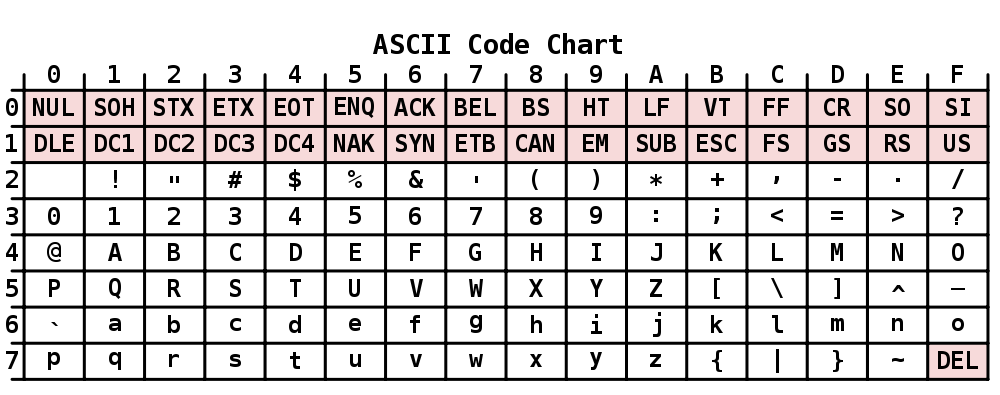
\includegraphics[scale=0.31]{img/1000px-ASCII_Code_Chart.png}

\vspace{-0.3cm}
{\scriptsize\hfill  Source: Wikimedia Commons, public domain.}
\end{frame}


\begin{frame}

  \begin{block}{Caractères}
\C{char c;\\
...\\
printf("Entrer un caractère$\backslash$n");\\
scanf("\%c", \alert{\&}c);
}
\\ \pause
    \alert{Attention :} mieux vaut utiliser
    \C{scanf("\textvisiblespace\%c", \alert{\&}c);}
  \end{block}\pause

\begin{block}{Chaînes de caractères}
\C{char nom[64];\\
...\\
printf("Entrer votre nom$\backslash$n");\\
scanf("\%s", nom);\\ \pause
}
\end{block}
\end{frame}


\subsection[Conversions automatiques]{Conversions automatiques entre types}
\begin{frame}[fragile]
  \frametitle{Conversions  automatiques entre types}

  \begin{itemize}
  \item Sans changement de représentation :
  \begin{itemize}
  \item \C{char} vers \C{int}
  \item \C{int} vers \C{char} (troncature)
  \end{itemize}\pause
  \begin{lstlisting}[basicstyle=\ttfamily\small]
  char c;
  int n;

  n = 'A' + 1; /* voir table ascii */
  c = n + 24; /* quel caractere vaut c ? */
\end{lstlisting}
 \item Avec changement de représentation :
    \begin{itemize}
    \item char ou entiers vers réels
    \item réels vers entiers ou char
    \end{itemize}
  \begin{lstlisting}[basicstyle=\ttfamily\small]
  double x;
  int n;

  n = 3.1; /* que vaut n ? */
  x = n;
   \end{lstlisting}
  \end{itemize}
\end{frame}

\section[Tableaux en C]{Mémoire et tableaux en C}
%\subsection{Mémoire et variables (rappels)}
\begin{frame}
  \frametitle{Mémoire et variables (rappels)\nowrite}
  \begin{itemize}
  \item Déclarer une variable a pour effet de réserver de la mémoire
    et de lui donner un usage particulier pour la suite du
    programme :\pause
    \begin{itemize}
    \item La déclaration \C{int toto;} aura pour effet de réserver l'espace mémoire nécessaire au stockage d'un entier.
\pause
\item  Dans la suite du programme, l'adresse de cet espace mémoire sera utilisée partout où il est fait référence à cette variable (identificateur \C{toto}).
\pause
\item C'est le codage machine des entiers en binaire qui sera employé pour manipuler cette donnée.
   \end{itemize}\pause
  \end{itemize}
  \begin{block}{Remarque.}
    La  taille d'un \C{int} est en principe exactement celle d'un mot
    mémoire, c'est à dire 4 ou 8 octets.
\end{block}
\end{frame}

\begin{frame}[fragile]
  \frametitle{Déclarations multiples et répétitives ?}
  \begin{lstlisting}
int main () {
    int i;
    /* repeter des declarations ? */
    for (i = 0; i < 1024; i = i + 1) {
        int X_i; /* marchera pas */
    }
    int somme = 0;
    /* saisie */
    for (i = 0; i < 1024; i = i + 1) {
        printf("X_i ?");
        scanf("%d", &X_i);
    }
    /* calcul */
    for (i = 0; i < 1024; i = i + 1) {
        somme  = somme + X_i;
    }
    return EXIT_SUCCESS;
}
  \end{lstlisting}
\pause
Solution : faire un tableau.
\end{frame}

\begin{frame}[fragile]
\frametitle{Solution : un tableau}
  \begin{lstlisting}
int main () {
    int i;
    int X[1024]; /* 1024 variables ! */
    int somme = 0;
    /* saisie */
    for (i = 0; i < 1024; i = i + 1) {
        printf("X[%d] ?", i);
        scanf("%d", &X[i]);
    }
    /* calcul */
    for (i = 0; i < 1024; i = i + 1) {
        somme  = somme + X[i];
    }
    return EXIT_SUCCESS;
}
  \end{lstlisting}
\end{frame}

\subsection{Déclaration d'un tableau en C}
\begin{frame}[fragile]
  \frametitle{Déclaration d'un tableau statique unidimensionnel}
  \begin{itemize}
\item    Du point de vue logiciel la mémoire se présente comme une
    succession d'octets, numérotés par les entiers à partir de
    $0$.
\pause
\end{itemize}
\begin{tabular}{r|c|c|c| c }
  \hline
  Adresses : & $0$ & $1$ & $2$ & \ldots \\ \hline
  octets (valeurs) :  & {\small 01000110} & {\small 11010111} & {\small 00000001} & \ldots \\
  \hline
\end{tabular}
\begin{itemize}
  \item En C, on peut réserver plusieurs espaces mémoires contigus pour des données de même type en une seule déclaration :\pause
    \begin{lstlisting}
      int toto[3];
    \end{lstlisting}
\end{itemize}
\pause
{
\scriptsize
\begin{tabular}{r| c| c|c|c|c| c|c|c|c| c|c|c|c| c}
  \hline
  Adresses : & \ldots & $344$ & & & & $348$& & & &  $352$& & & & \ldots \\ \hline
  Valeur :  & \ldots & \multicolumn{4}{|c|}{{\tiny 1 \ldots0}}
                              & \multicolumn{4}{|c|}{{\tiny 0\ldots1}}
                              & \multicolumn{4}{|c|}{{\tiny 1\ldots1}} & \ldots \\
\hline
\uncover<6->{\emph{Identificateur}: & \ldots & \multicolumn{4}{|c|}{\C{toto[0]}} &  \multicolumn{4}{|c|}{\C{toto[1]}} &  \multicolumn{4}{|c|}{\C{toto[2]}} & \ldots  }
\end{tabular}\medskip
}
  \begin{itemize}
    \item La taille doit être connue à la compilation\pause
    \item Les cases sont accessibles, comme s'il s'agissait de variables, à l'aide des identificateurs \C{toto[0]}, \C{toto[1]}, \C{toto[2]}\pause
    \item   La numérotation commence à zéro. Si $n$ est la taille la dernière case est donc numérotée $n - 1$.
  \end{itemize}
\end{frame}

\begin{frame}
  \frametitle{Attention !}
  \begin{alertenv}
Il ne faut jamais accèder à une case au delà de la numérotation : \C{toto[3]}, \C{toto[-1]}, etc. Le compilateur ne vous préviendra pas de votre erreur, mais le programme va boguer.
\end{alertenv}
\pause

L'erreur d'exécution \C{segmentation fault} signifie que le programme
a effectué un accès à une case mémoire qui ne lui était pas réservée
(mais il faut beaucoup s'écarter des bons indices du tableau).
\end{frame}

%\subsection{Exemples et trace}
\begin{frame}[fragile]
  \frametitle{Premier exemple}
\begin{lstlisting}[escapechar={\%},basicstyle=\ttfamily]
int main()
{
  /*Declaration et initialisation de variables*/
  int tableau[3]%\only<3>{\colorbox{yellow}{= \{3,5,8\}}}%;

  tableau[0] = 3; %\only<3>{\emph{$\leftarrow$ inutile}}%
  tableau[1] = 5; %\only<3>{\emph{$\leftarrow$ inutile}}%
  tableau[2] = tableau[0] + tableau[1]; %\only<3>{\emph{$\leftarrow$ inutile}}%

  return EXIT_SUCCESS;
}
\end{lstlisting}
\end{frame}

\begin{frame}[fragile]
  \frametitle{Second exemple}
\begin{lstlisting}[basicstyle=\ttfamily\small]
int main()
{
  /* Declaration et initialisation de variables */
  int tab[3] = {3,5,8};
  int i; /* var. de boucle */
\end{lstlisting}
\pause
\begin{lstlisting}[basicstyle=\ttfamily\small]
  for (i = 0; i < 3; i = i + 1) /* pour chaque case */
  {
    printf("tab[%d] = %d\n", i, tab[i]);
  }
  return EXIT_SUCCESS;
}
\end{lstlisting}
\end{frame}

\begin{frame}[fragile]
  \frametitle{Trace du second exemple}

\begin{lstlisting}[numbers=left,basicstyle=\ttfamily\tiny]
int main()
{
  /* Declaration et initialisation de variables */
  int tab[3] = {3,5,8};
  int i; /* var. de boucle */

  for (i = 0; i < 3; i = i + 1) /* pour chaque case */
  {
    printf("tab[%d] = %d\n", i, tab[i]);
  }
  return EXIT_SUCCESS;
}
\end{lstlisting}

 \scriptsize
\pause
\rowcolors[\hline]{2}{green!25}{yellow!50} \arrayrulecolor{blue!75!gray}
  \begin{tabular}{|r|c|c|c|c|l|}
\hline
    ligne & \C{tab[0]} & \C{tab[1]} & \C{tab[2]} & \C{i} & sortie
    écran  \pause \\
   initialisation & 3 & 5 & 8 & ? &  \pause \\
7 & & & & 0 & \pause \\
 9 & & & &  & \C{tab[0] = 3} \pause  \\
  10 & & & & 1 & \pause \\
  9 & & & &  & \C{tab[1] = 5} \pause \\
 10 & & & & 2 & \pause \\
  9 & & & &  & \C{tab[2] = 8} \pause \\
 10 & & & & 3 & \pause \\
11 & \multicolumn{4}{c}{Renvoie \C{EXIT\_SUCCESS}} & \\
  \end{tabular}
\end{frame}

\subsection{Les tableaux : une structure de données}
\begin{frame}
  \frametitle{La structure de donnée tableau}
    Les tableaux sont une manière très naturelle d'organiser
    des données de même type. \structure{Beaucoup d'algorithmes utilisent des tableaux.}
\pause
  \begin{itemize}
\item On peut accéder très rapidement à
  n'importe quel élément si on connaît son indice,
on peut aussi  très simplement parcourir un tableau;
 \item supprimer ou insérer un élément sont des opérations
    plus lentes, comme y chercher un élément si le tableau n'est pas préalablement
    classé dans un certain ordre. \pause \alert{Connaissez vous la recherche
    dichotomique ?}\pause
\item Classer un tableau peut prendre plus de temps, parce que
  classer des éléments prend du temps qu'ils
    soient sous forme de tableau ou non. \pause \alert{Connaissez vous un
    algorithme de tri (rangement sous forme classée) ?} Exploite t'il
    la structure de tableau ou une autre structure ?
  \end{itemize}
\end{frame}

\section[Chaînes]{Les chaînes de caractères}
\begin{frame}[fragile]
  \frametitle{Les chaînes de caractères}
  \begin{itemize}
    \item Une chaîne de caractère est un tableau de caractère, terminé
      par le caractère spécial de code ascii zéro (on parle de
      sentinelle), \alert{\C{$\backslash 0$}}.
\item Plutôt que d'écrire :
  \begin{lstlisting}
char nom[7] = {'m','o','n',' ','n','o','m'};
  \end{lstlisting}
\item on peut utiliser directement :
  \begin{lstlisting}
char nom[8] = "mon nom";
  \end{lstlisting}
\item Le huitième caractère, \C{$\backslash 0$} sert à délimiter le
  texte.
\item On peut même écrire :
  \begin{lstlisting}
char nom[] = "mon nom";  /* 8 cases */
  \end{lstlisting}
\item Avec printf et scanf  on utilise \C{\%s}.
\item Pour les entrées on utiliser surtout  \C{fgets} :
  \begin{lstlisting}
fgets(nom, 64, stdin); /* lit 63 car. maxi */
  \end{lstlisting}
  \end{itemize}
\end{frame}

\section{Les enregistrements (struct)}

\begin{frame}[fragile]
  \frametitle{Autre problème de données multiples}
\begin{verbatim}
Entrer la première fraction : -1 / 42
...
\end{verbatim}
\pause
Quel type de sortie donner à la fonction de saisie utilisateur d'une
fraction ? Une fonction retourne une seule valeur !
\pause
  \begin{lstlisting}
int[2] saisir_fraction(); /* error: (syntaxe) */
int * saisir_fraction(); /* probleme memoire */
  \end{lstlisting}
\pause
 Il nous faut \emph{empaquetter} ces deux entiers en une seule valeur.
\end{frame}

\begin{frame}
  \frametitle{Les enregistrements ou  « struct »}
\begin{itemize}
\item Une structure \emph{empaquette} plusieurs valeurs nommées et s'utilise comme un \alert{type}. \pause
\item Chacune des valeurs est accessible à l'aide d'un nom, choisi au
  moment de  la  déclaration de la structure. On parle des \alert{champs} de la
  structure.\pause
\item Un type structure doit être déclaré avant d'être
  utilisé. Ne pas confondre : \textbf{déclaration de variable} (dans une
  fonction), \textbf{déclaration de type structure} et  \textbf{déclaration de fonction}.
\pause
\item Les valeurs des champs sont accessibles individuellement à l'aide de la
  \alert{notation pointée}. \pause
\item On peut aussi manipuler globalement la valeur d'une donnée de
  type structure. Par exemple : faire une affectation entre variables
  d'un même type structure (copie les champs, y compris les tableaux statiques).
\end{itemize}
\end{frame}

\subsection[Déclaration]{Déclaration d'un type struct}
\begin{frame}[fragile]
  \frametitle{Déclaration d'un type struct}
\begin{lstlisting}[escapechar={\%},basicstyle=\ttfamily\small]
struct bulletin_s  {
  double temperature; /* temperature de l'air */
  int force;          /* force du vent (Beaufort) */
}; /* <-- attention ';' (cas particulier) */
\end{lstlisting}
\pause
\begin{itemize}
\item Cette déclaration est placée en dehors de toute fonction, entre
les définitions de constantes symboliques (\verb|#define ...|) et les
déclarations de fonctions utilisateur.
\pause
\item L'effet de cette déclaration est de signaler au compilateur qu'un nouveau
type est disponible et comment il peut être utilisé (liste des champs). Aucun espace mémoire n'est réservé à ce moment
(ce n'est pas une déclaration de variable).
\item \pause \alert{Attention au point-vigule final}.
\end{itemize}
\end{frame}

\subsection[Utilisation]{Utilisation d'un type struct}
\begin{frame}[fragile]
  \frametitle{Utilisation d'un type struct: variables}

\begin{lstlisting}[escapechar={\%},basicstyle=\ttfamily\small]
int main()
{
    struct bulletin_s x = {0.5, 4};
    struct bulletin_s y;

    y = x; /* copie globale */
    x.temperature = 13.4; /* modif. d'un champ */
    ...
}
\end{lstlisting}
\pause
\begin{itemize}
\item Initialisation:  syntaxe proche de celle des tableaux.
\pause
\item la déclaration d'une variable de type structure reprend le mot
  clé \verb|struct| et le nom donné à la structure.
\pause
\item On accéde aux éléments d'une structure à l'aide de la notation
  pointée :
\verb|nom_variable.nom_champ|
\end{itemize}
\end{frame}

%\section{Type struct et fonctions (utilisateur)}
\begin{frame}[fragile]
  \frametitle{Utilisation d'un type struct: fonctions}

\begin{lstlisting}[escapechar={\%},basicstyle=\ttfamily\small]
/* declaration de fonctions utilisateur */
struct bm_s moyenne_bm(struct bm_s x, struct bm_s y);
\end{lstlisting}
\pause
On emploie \verb|struct nom_struct|, comme pour une déclaration de variable.
\begin{lstlisting}[escapechar={\%},basicstyle=\ttfamily\small]

/* definitions des fonctions utilisateur */
struct bm_s moyenne_bm(struct bm_s x, struct bm_s y)
{
    struct bm_s nouveau_bm;

    nouveau_bm.temperature = (x.temperature
                              + y.temperature) / 2.0;
    nouveau_bm.force = (x.force + y.force) / 2;

    return nouveau_bm;
}
\end{lstlisting}
\end{frame}

\begin{frame}[fragile]
  \frametitle{Avec typedef}
  On utilise souvent \alert{typedef} pour se passer du mot clé struct et
  donner un véritable nom de type à la structure.

\begin{lstlisting}
typedef struct bm_s {
   double temperature;
   int force;
} bm_t; /* <-- bm_t === struct bm_s */

bm_t moyenne_bm(bm_t x,  bm_t y);
\end{lstlisting}
\end{frame}

%\subsection[Intérêt]{Intérêt des structures (enregistrements)}
\begin{frame}
  \frametitle{Intérêt des structures (enregistrements)}

Intérêt des structures  :
  \begin{itemize}
   \item \structure{Lisibilité} : regrouper un ensemble
      de données dans un même type, nommé de façon explicite,
      facilite la relecture du code;\pause
  \item \structure{Augmente les possibilités} : les structures permettent d'écrire des
    fonctions qui retournent plusieurs valeurs, en l'absence de pointeurs.\pause
    \item \structure{Modularité} : on peut rajouter des champs très
      facilement, avec très peu de modifications.\pause
    \item \structure{Incontournables :} les langages orientés objets
      généralisent la notion de structure. Un objet est une structure
      dont les champs peuvent être aussi bien des données que des
      fonctions (hors programme).
  \end{itemize}
\end{frame}



%\subsection[Quelques erreurs]{Quelques erreurs communes}
\begin{frame}[fragile]
  \frametitle{Erreurs communes}

\begin{itemize}
\item Message d'erreur \emph{étrange} :
\begin{lstlisting}[numbers=left,basicstyle=\ttfamily\small,firstnumber=7]
struct bm_s  {
  double temperature; /* temperature de l'air */
  int force;          /* force du vent (Beaufort) */
}

/* Declaration des fonctions utilisateur */
void afficher_bm(struct bm_s);
\end{lstlisting}
{\small
\begin{verbatim}
14: error: two or more data types in declaration specifiers
\end{verbatim}
}
\pause
\alert{Oubli du point-virgule !}
\pause
\item Champ inexistant :
\begin{lstlisting}[numbers=left,basicstyle=\ttfamily\small,firstnumber=22]
  x.toto = 3; /* erreur: pas de champs toto */
\end{lstlisting}
{\small
\begin{verbatim}
prog.c: In function ‘main’:
prog.c:22: error: ‘struct bm_s’ has no member named ‘toto’
\end{verbatim}
}
\end{itemize}
\end{frame}

\section{Conclusion}
\begin{frame}
  \frametitle{Conclusion}
  \begin{itemize}
  \item On dispose d'entiers \C{int}, (et de booléens \C{bool}), de
    caractères \C{char}, et de nombres à virgule \C{double}. Pour le
    reste, on peut créer de nouveaux types avec les tableaux et
    surtout les structures.\pause
  \item Un tableau est un \alert{lot de  variables
      identiques numérotées}.\pause
  \item Une \alert{chaîne de caractères} est un tableau de \C{char} où le
    caractère \C{'$\backslash 0$'} représente la fin de la chaîne.
  \item Une structure  \alert{regroupe
      des variables  de différents types},
    dûment nommées. \pause
  \item Pour les tableaux (ou les chaînes) comme pour les structures,
    on ne peut pas utiliser les opérations usuelles : comparaisons, test
    d'égalité, opérations arithmétiques. Il faut introduire des
    fonctions spécifiques.
  \end{itemize}
  \end{frame}
\end{document}

% revenir sur :
%-l'appel au cours suivant : paramètre et expression, pile d'appel.
%-la grammaire des identificateurs